\documentclass[pdftex,12pt,a4paper]{article}
\usepackage[utf8]{inputenc}
\usepackage[T1]{fontenc}
\usepackage{lmodern}
\usepackage{tabularx}
\usepackage{multirow}
\usepackage{graphicx}
\usepackage{hyperref}
\usepackage[ngerman]{babel}
\usepackage{booktabs,paralist}
\usepackage{scrpage2,lastpage}
\usepackage{a4wide}
\begin{document}
\newcommand{\half}{0.5\textwidth}

% Titelblatt
\begin{titlepage}
\begin{center}
\textsc{\LARGE Technische Universit\"at Dresden} \\[0.5cm]
\textsc{\LARGE Softwaretechnologie-Projekt\\[0.2cm]Gruppe 30}\\[0.7cm]
\textsc{\LARGE Geek-Shop}\\[4cm]
{\fontsize{35}{35} \bfseries Benutzerhandbuch}\\
\vspace*{\fill}
Sebastian D\"oring, Felix D\"oring, Marcus Kammerdiener,\\ Dominik Lauck, Elizaveta Ragozina\\[0.5cm]
\url{http://is63050.inf.tu-dresden.de/~swt14w30/index.php}
\end{center}
\end{titlepage}


% Inhaltsverzeichnis
\tableofcontents
\newpage

% Einführung und Ziele
\section{Einf\"uhrung und Ziele}

% Aufgabenstellung
\subsection{Aufgabenstellung} 
\textbf{„Think Nerd“ – The Shop for your nerdy needs.}\\[.25cm]
Ein echter Computer-Nerd hat ganz besondere Bedürfnisse. Wir wissen das selbst am besten. Daher haben wir uns entschlossen, einen Shop zu eröffnen, der von einfachen koffeinreichen Minzpastillen über das monatliche Linuxmagazin bis hin zur Armbanduhr mit WLAN-Empfänger alles Wichtige anbietet. „Think Nerd“ ist dabei nicht nur ein Name, sondern vielmehr unsere Geschäftsphilosophie. Schnell war klar, wir wollen ein eigens für uns entwickeltes Verwaltungssystem. Das Programm soll primär an der Kasse eingesetzt werden und den Verkaufsvorgang elektronisch abwickeln können. Bei uns gibt es nur normale Angestellte und den Ladenbesitzer.\\
Um das Geschäftsklima zu verbessern, hätten wir gern, dass jeder Angestellte mit einem zufälligem Nerd-Witz begrüßt wird. Damit sich die Witze nicht ständig wiederholen, soll der Ladenbesitzer die Möglichkeit haben, Witze entsprechend zu verwalten.\\
Einzelne Mitarbeiter sollen sich mit ihrem Namen und einem sicheren Passwort anmelden können. Unsichere Passwörter sollen bei uns gar nicht erst zugelassen werden. Ein Passwort wie „mama“ wäre also unerwünscht. Möglich wäre z. B. „MaM4.12\$“.\\
Mitarbeiter sollen vor allem Einkäufe von Kunden abwickeln. Unser Sortiment ist in Kategorien wie z. B. „Nerd-Wear“ oder „Elektronische Gagdets“ gegliedert. Die Kategorien sind ihrerseits wieder in Unterkategorien wie z. B. „Admin-Shirts“ o. „Gamer-Shirts“ unterteilt. Mitarbeiter sollen sich zunächst durch das Sortiment „klicken“ können oder über eine Suchfunktion Waren direkt finden. Angezeigte Ergebnisse sollen nach allen Kriterien (auf/absteigend nach Preis, nach Name ...) sortiert werden können, wie man es von gängigen Online-Shops her kennt. Die Angestellten sollen die Möglichkeit haben, die Waren nacheinander in einen Warenkorb einzufügen. Im nächsten Schritt sollen die Angestellten eine Übersicht über den Einkauf erhalten und die Zahlungsweise eingeben können. Es ist für Kunden möglich per elektronischem Lastschriftverfahren, per Kreditkarte oder bar zu zahlen. Nach der Bezahlung soll eine druckfertige Rechnung angezeigt werden.\\
Wir haben eine 14-tägige Geld-zurück-Garantie. Falls ein Kunde etwas reklamieren möchte, soll(en) der/die Artikel ebenfalls in einen Warenkorb gelegt werden. Im nächsten Schritt soll noch einmal die Übersicht über die Reklamation gezeigt werden. Es ist dann erforderlich, dass der Abschluss einer Reklamation vom Ladenbesitzer genehmigt werden muss. Am besten wäre es, wenn er dazu Name und Passwort eingeben müsste.\\
Der Ladenbesitzer ist für die Verwaltung der Mitarbeiter zuständig. Er kann sie entlassen, einstellen oder ihre persönlichen Daten verändern. Nur der Ladenbesitzer kann das Sortiment bearbeiten. Das hei\ss{}t er kann Kategorien und Unterkategorien erstellen, löschen und umbenennen. Ebenfalls kann nur er Artikel hinzufügen, löschen und bearbeiten.\\
Ein Überblick über den aktuellen Lagerbestand ist ebenfalls erforderlich. Der Ladenbesitzer muss den Bestand natürlich auch verändern können, um neue Lieferungen einzutragen.\\
Wenn der Bestand eines Artikels eine untere Grenze unterschreitet, möchte der Ladenbesitzer natürlich gewarnt werden.\\
Der Ladenbesitzer kann auf „Rohdaten“ aller Verkäufe zugreifen. Also wann, welcher Artikel, in welcher Menge verkauft wurde. Wir planen bei einem Freelancer ein umfangreiches Statistik-Tool für uns in Auftrag zu geben. Damit dieser gleich diese Rohdaten benutzen kann, brauchen wir eine Exportfunktion, die die Daten in eine XML Datei schreibt.

% Stakeholder
\subsection{Stakeholder}
\begin{tabularx}{\textwidth}{| *4{>{\arraybackslash}X|}} \hline
{\textbf{Rolle}} & {\textbf{Beschreibung}} & {\textbf{Ziel/Intention}} & {\textbf{Bemerkungen}}\\ \hline
Owner & Ladenbesitzer & GELD & alle Rechte\\ \hline
Employee & Mitarbeiter & Arbeiten $\rightarrow$ Geld & Sklave\\ \hline
\end{tabularx}

% Randbedingungen
\section{Randbedingungen}
% Technische Randbedingungen
\subsection{Technische Randbedingungen}
\begin{tabular}{|p{\half}|p{\half}|} \hline
\multicolumn{2}{|p{\textwidth}|}{Hardware-Vorgaben}\\ \hline
& RAM: 128 MB\\ \cline{2-2}
& Datentr\"agerkapazit\"at: 150 MB\\ \cline{2-2}
& mindestens 266MHz-Prozessor\\ \hline
\multicolumn{2}{|p{\textwidth}|}{Software-Vorgaben}\\ \hline
& Java 8\\ \cline{2-2}
& Browser mit HTML5-Unterst\"utzung\\ \hline
\multicolumn{2}{|p{\textwidth}|}{Programmiervorgaben}\\ \hline
& Java 8\\ \cline{2-2}
& Thymeleaf\\ \cline{2-2}
& Maven 3.2.5\\ \cline{2-2}
& Spring-Framework 4.1.4\\ \cline{2-2}
& SalesPoint-Framework 6.1.1\\ \hline


\end{tabular}



% Konventionen
\subsection{Konventionen}
Zur optischen Unifizierung des Codes und zur Optimierung der {\textit{Imports}} wurde die Autoformatierung von IntelliJ IDEA 14 verwendet.\\
Die Namenskonvention lautet wie folgt:\\
\begin{itemize}
\item Klassennamen beginnen mit einem Gro\ss{}buchstaben, bestehen sie aus mehreren W\"ortern, so werden sie zusammen geschrieben und jeweils der erste Buchstabe gro\ss{}
\item Methodennamen beginnen mit einem Kleinbuchstaben, bestehen sie aus mehreren W\"ortern, so werden sie zusammen und ab dem zeiten Wort die Anfangsbuchstaben gro\ss{} geschrieben.
\end{itemize}

% Kontextabgrenzung
\newpage
\section{Kontextabgrenzung}

% Fachlicher Kontext
\subsection{Fachlicher Kontext}
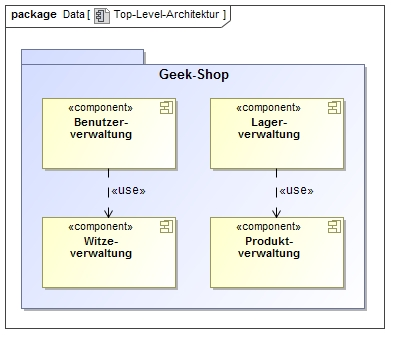
\includegraphics[width=\textwidth]{../Pflichtenheft/images/toplevelarchitektur}


% Technischer oder Verteilungskontext
\subsection{Technischer oder Verteilungskontext}

% Externe Schnittstellen
\subsection{Externe Schnittstellen}

% Lösungsstrategie und Entwurfsentscheidungen
\section{Lösungsstrategie und Entwurfsentscheidungen}

% Bausteinsicht
\section{Bausteinsicht}

% Laufzeitsicht
\section{Laufzeitsicht}

% Persistenz
\subsection{Persistenz}

% Benutzungsoberfläche
\subsection{Benutzungsoberfläche}

% Ergonomie
\subsection{Ergonomie}

% Transaktionsbehandlung
\subsection{Transaktionsbehandlung}

% Sessionbehandlung
\subsection{Sessionbehandlung}

% Sicherheit
\subsection{Sicherheit}

% Plausibilisierung und Validierung
\subsection{Plausibilisierung und Validierung}

% Ausnahme-/Fehlerbehandlung
\subsection{Ausnahme-/Fehlerbehandlung}

% Logging, Protokollierung, Tracing
\subsection{Logging, Protokollierung, Tracing}

% Konfigurierbarkeit
\subsection{Konfigurierbarkeit}

% Internationalisierung
\subsection{Internationalisierung}

% Testbarkeit
\subsection{Testbarkeit}

% Buildmanagement
\subsection{Buildmanagement}

% Glossar
\section{Glossar}


\end{document}